



\documentclass[twocolumn]{article}
\usepackage{graphicx}
\usepackage{subfig}
\usepackage{lipsum}

%\captionsetup{skip=<15mm}
%\captionsetup[subfloat]{captionskip=40pt}
\begin{document}
%    \section{Introduction}
%    \lipsum[1-5]
    \thispagestyle{empty}
    \begin{figure*}[t!]
                \captionsetup[subfigure]{font=Large}

        \subfloat[]{%
            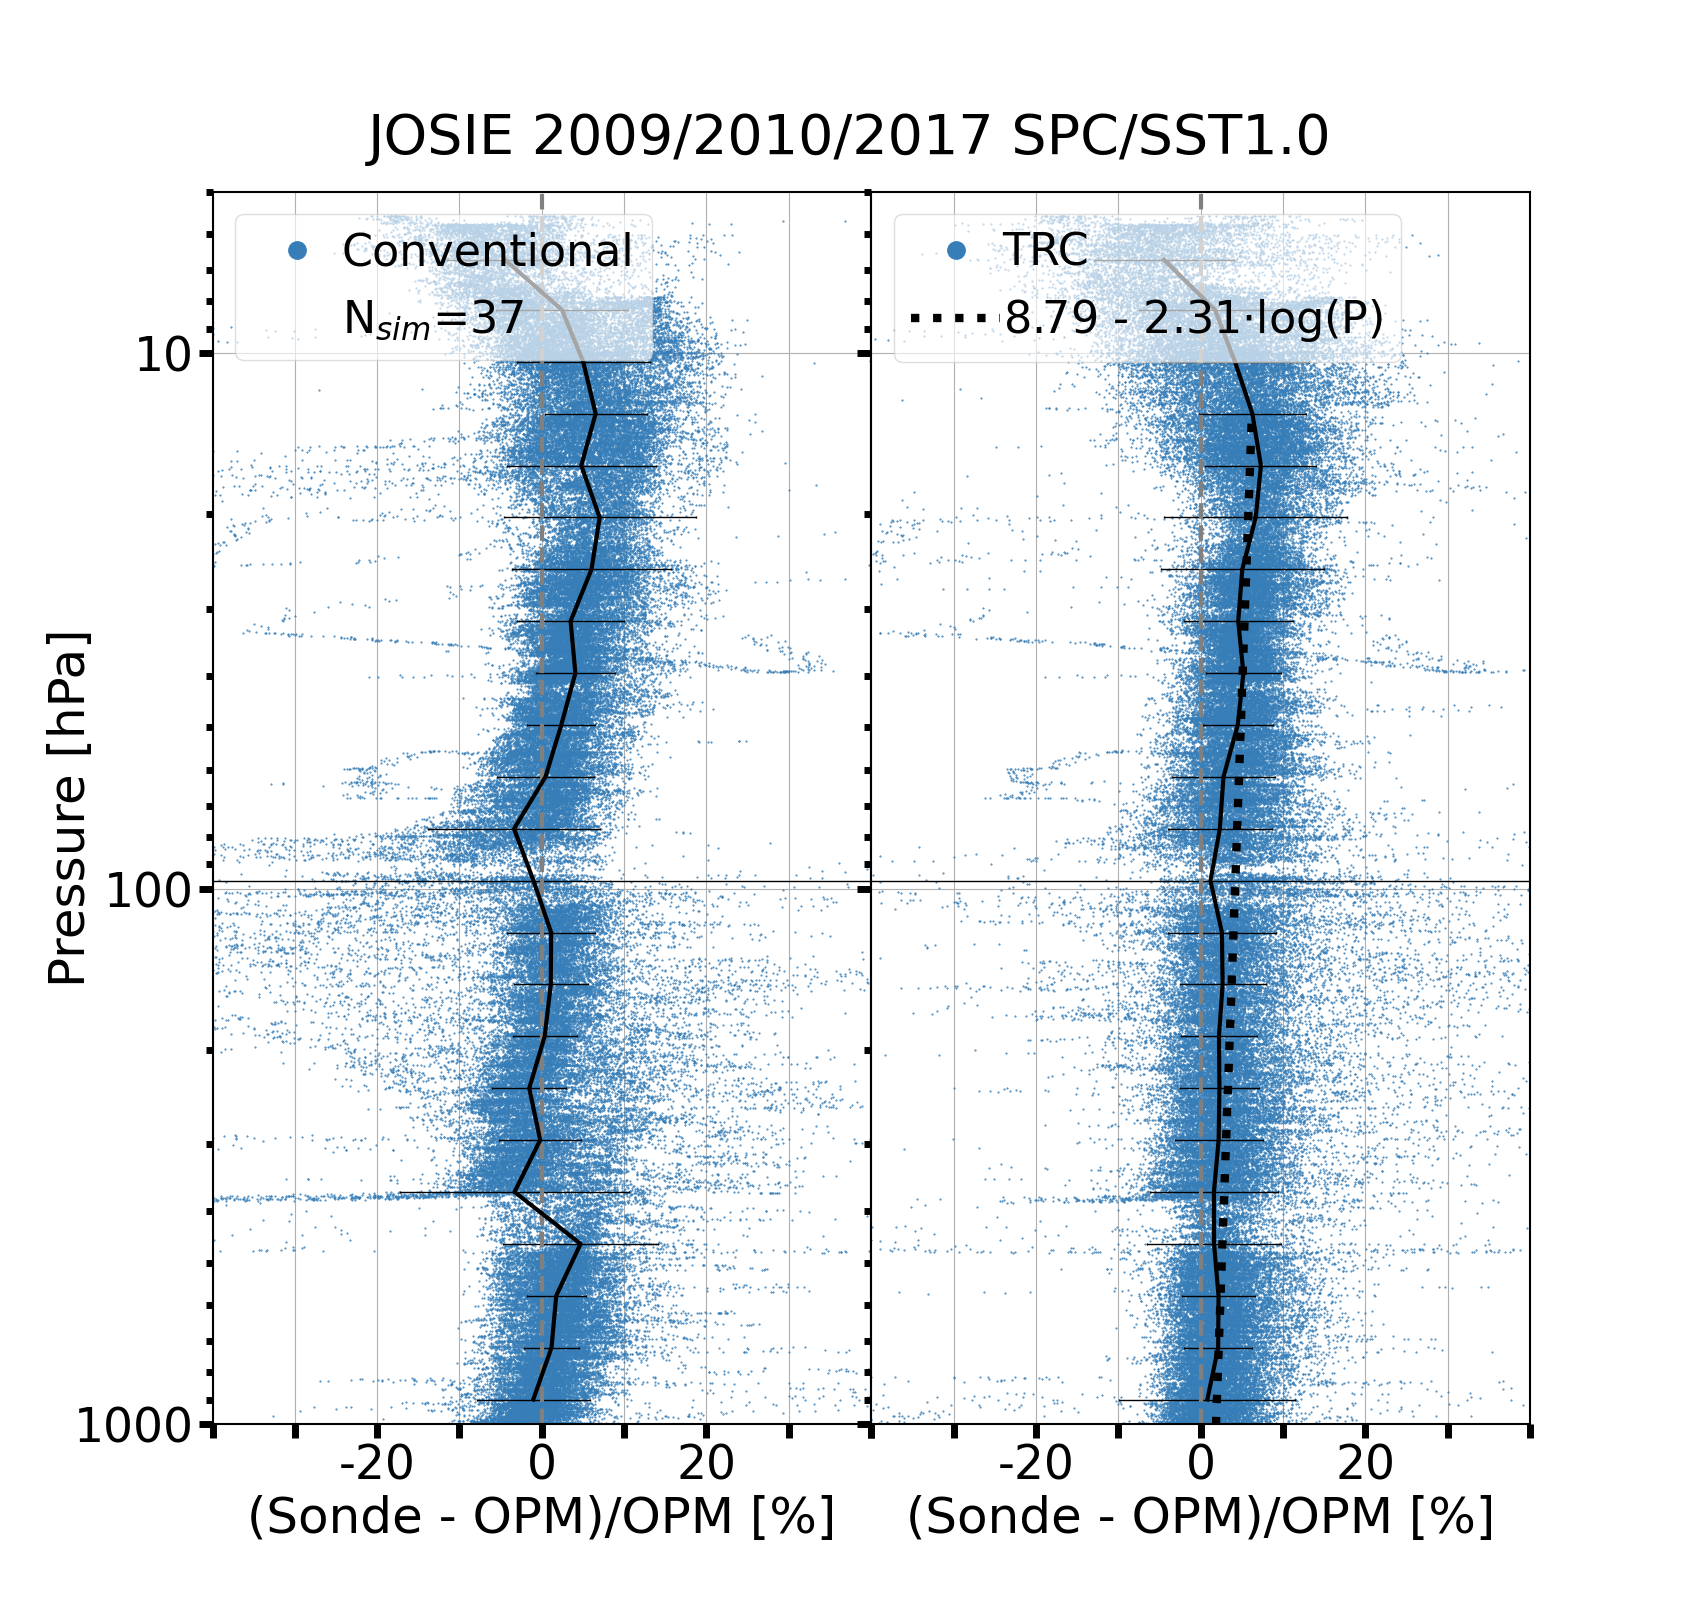
\includegraphics[width=.63\linewidth]{png/scatter_all__0910-2017_SPC1010_pressure}%

%            \label{subfig:a}%
        }
        \hspace{-9mm}
        \subfloat[]{%
            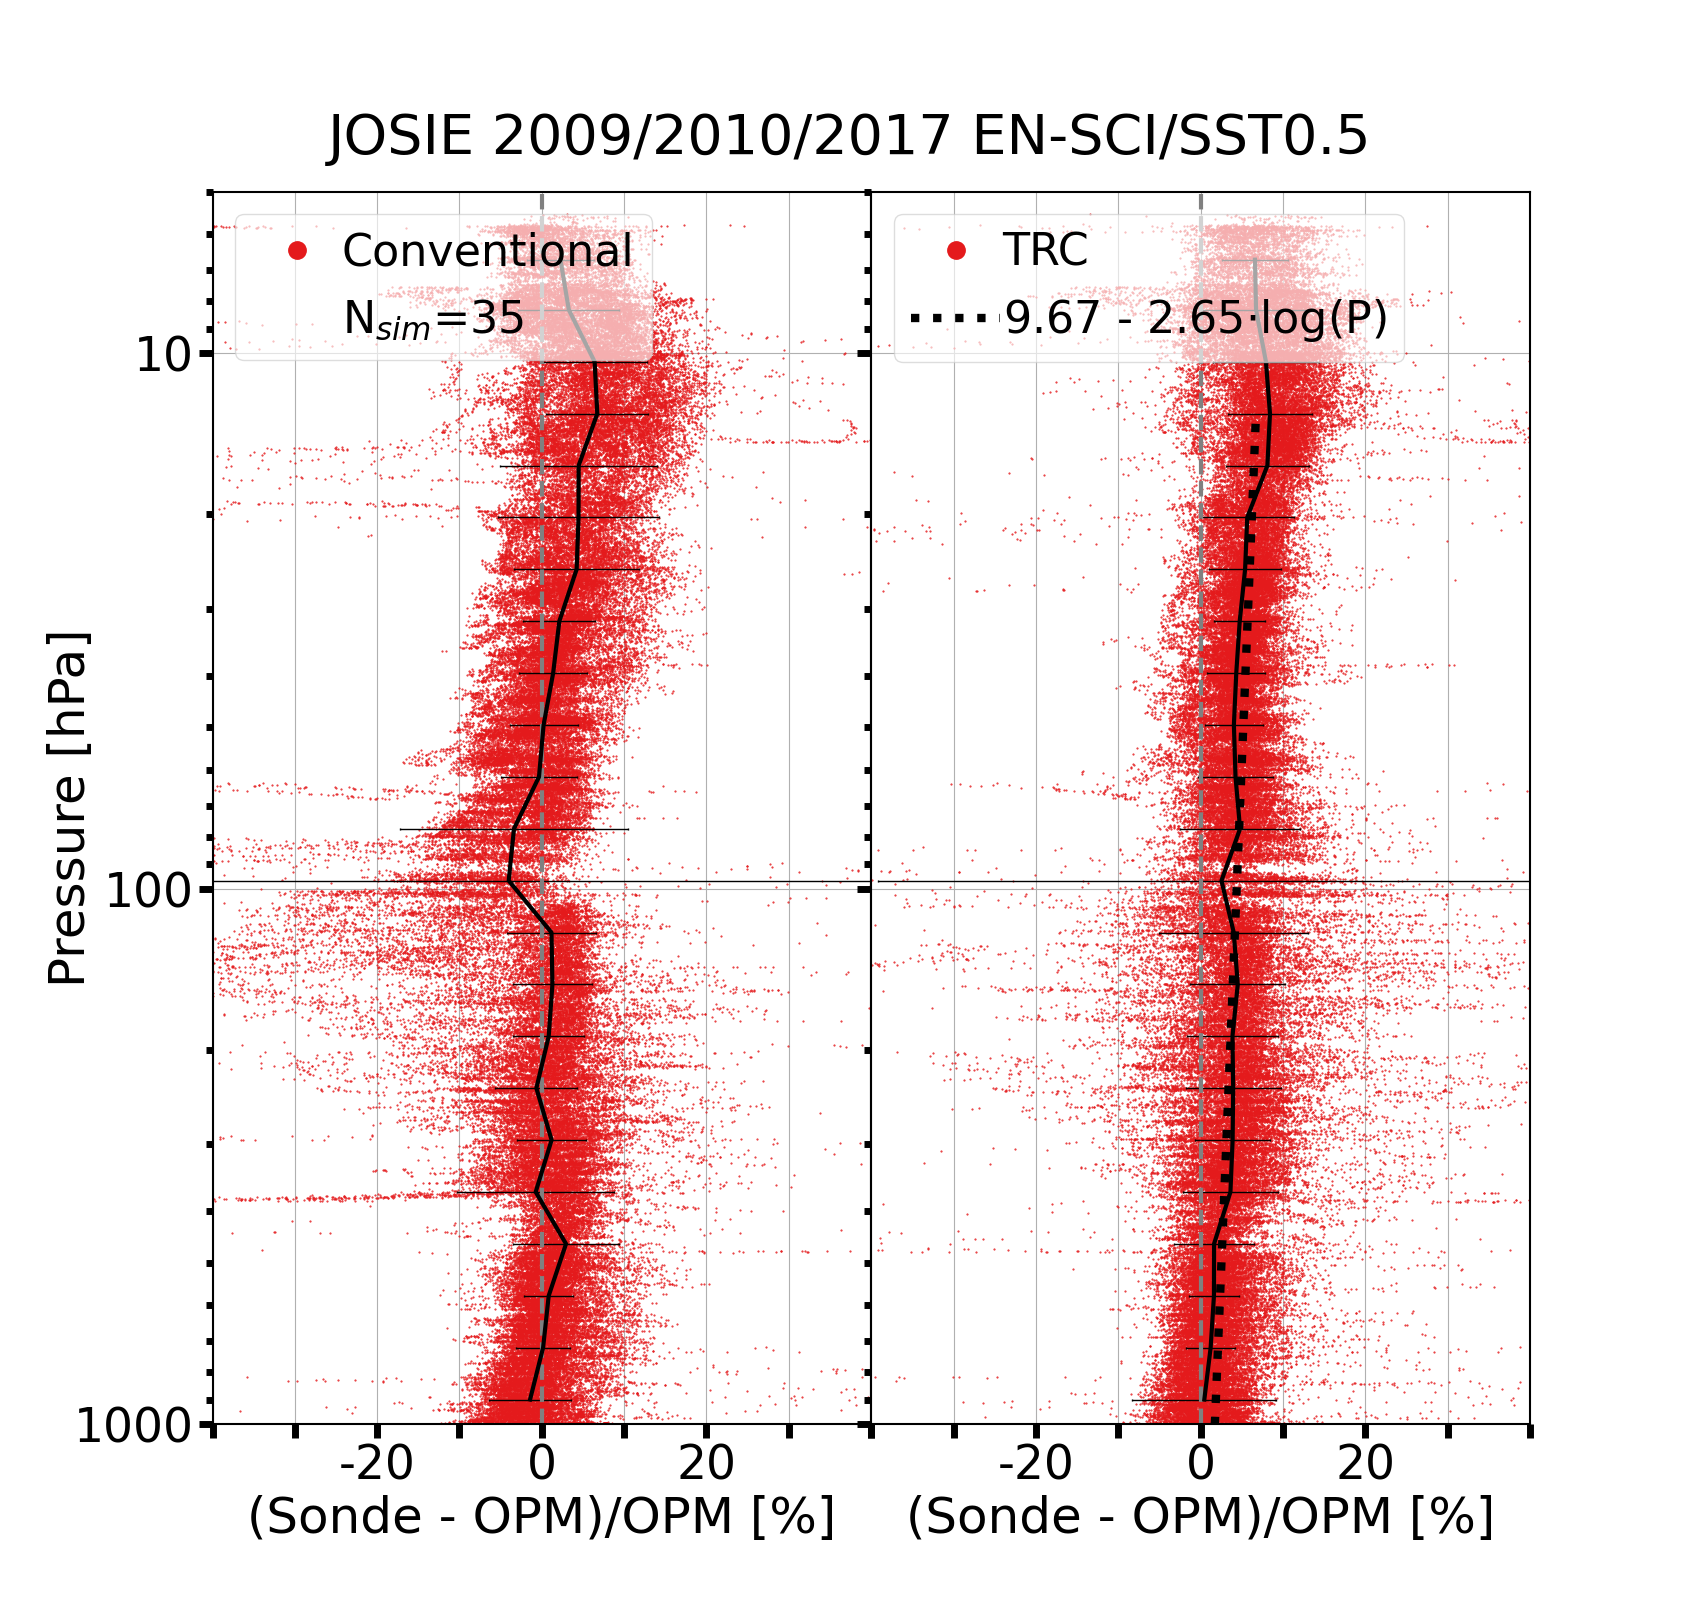
\includegraphics[width=.63\linewidth]{png/scatter_all__0910-2017_EN0505_pressure}%
            \label{subfig:b}%
        }
        \hspace{0mm}

    \end{figure*}
\end{document}







%
%
%
%
%\documentclass[twocolumn]{article}
%\usepackage{graphicx}
%\usepackage{subfig}
%\usepackage{lipsum}
%
%\begin{document}
%%    \section{Introduction}
%%    \lipsum[1-5]
%    \thispagestyle{empty}
%    \begin{figure*}[t!]
%        \subfloat[]{%
%            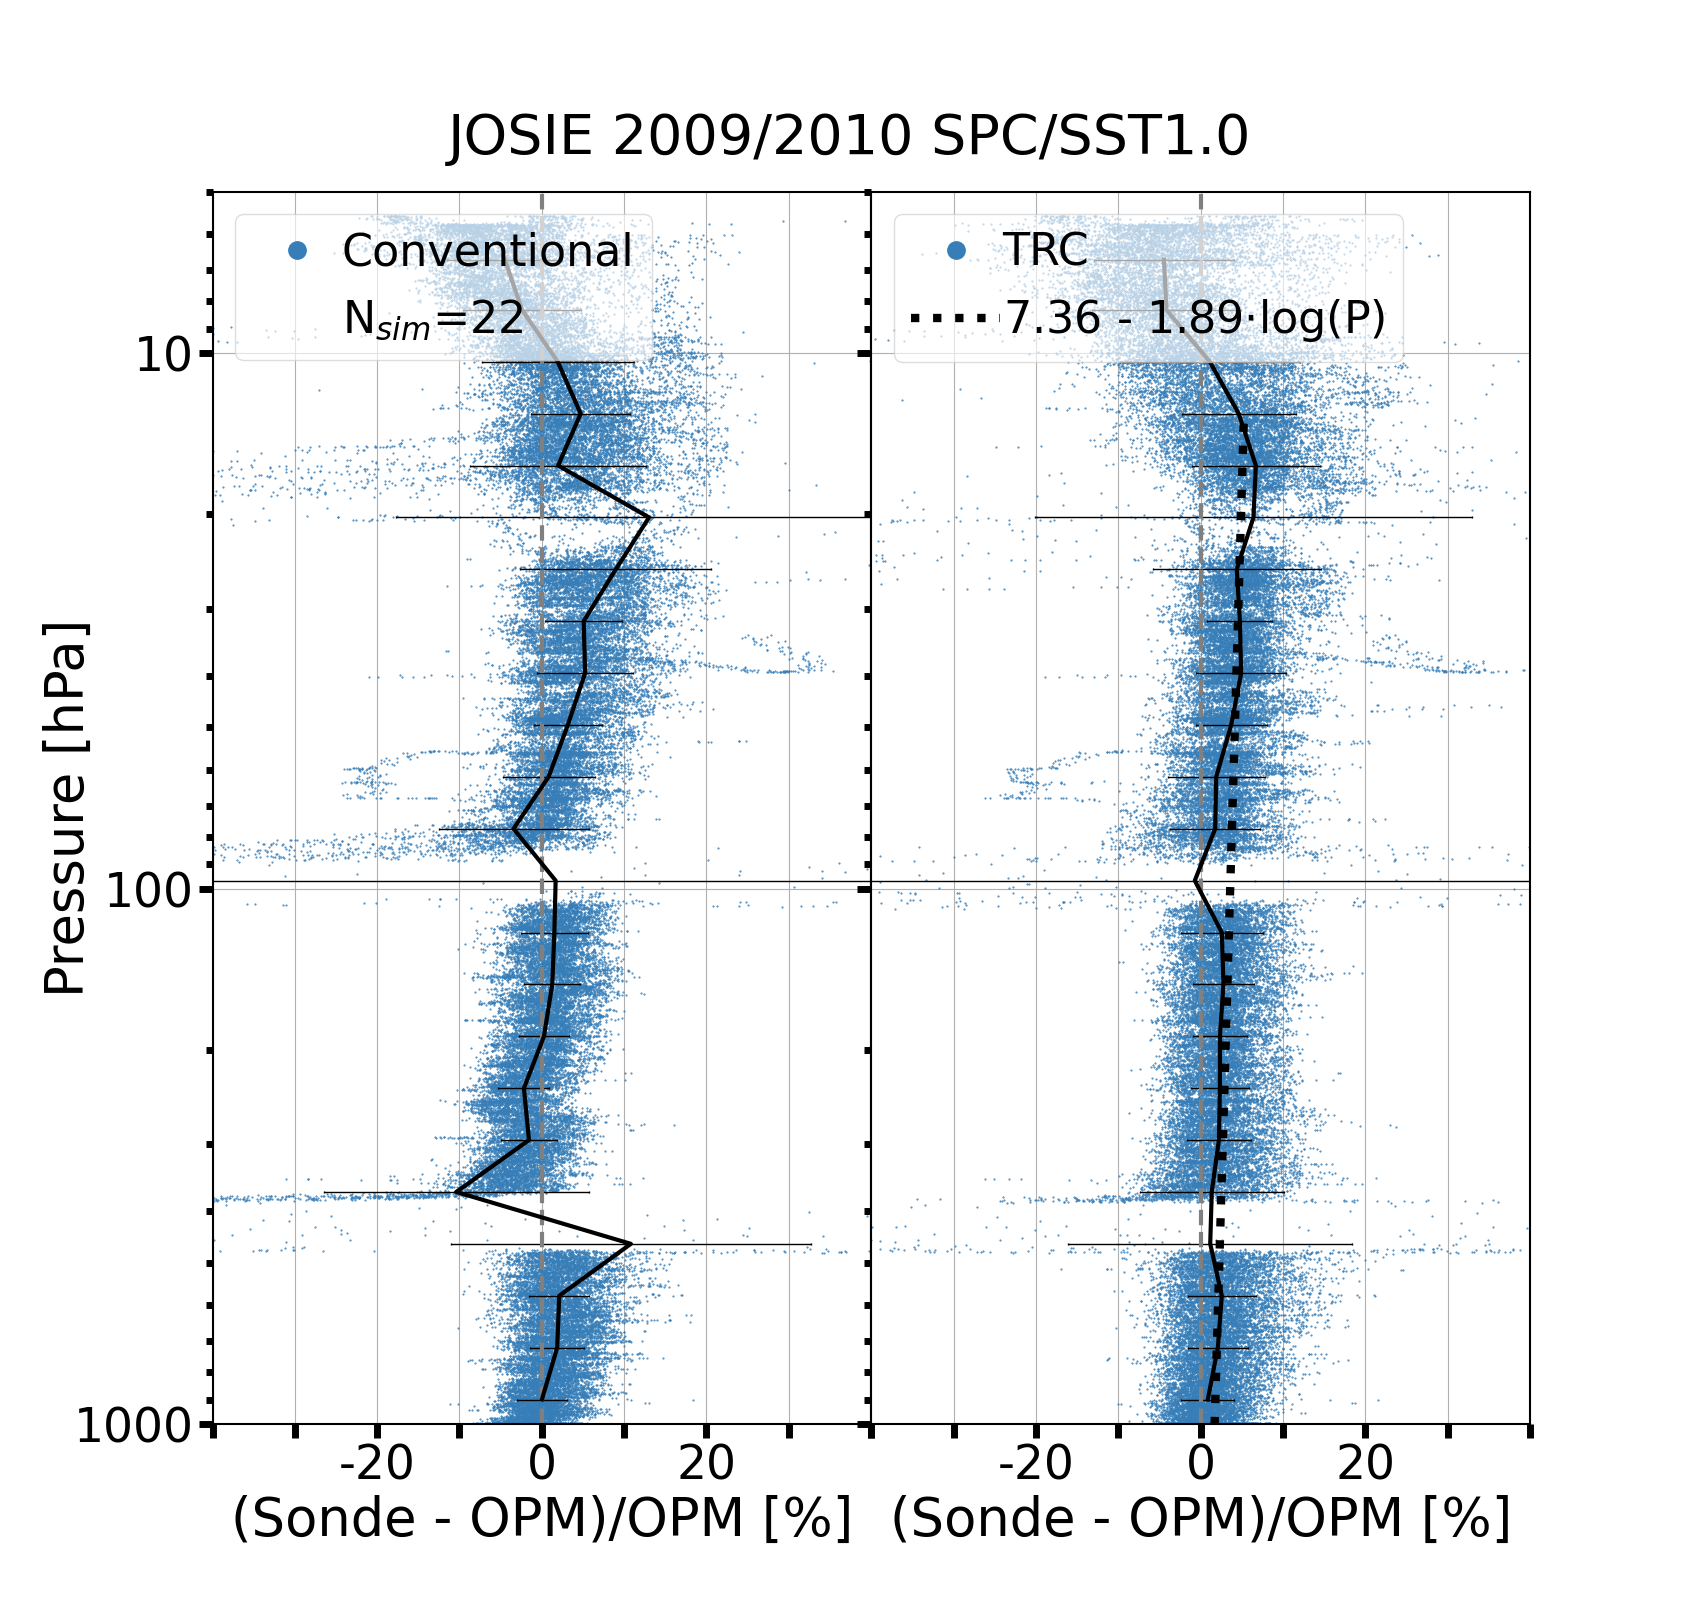
\includegraphics[width=.48\linewidth]{png/scatter_fig6_0910_SPC1010_pressure}%
%            \label{subfig:a}%
%        }\hfill
%        \subfloat[]{%
%            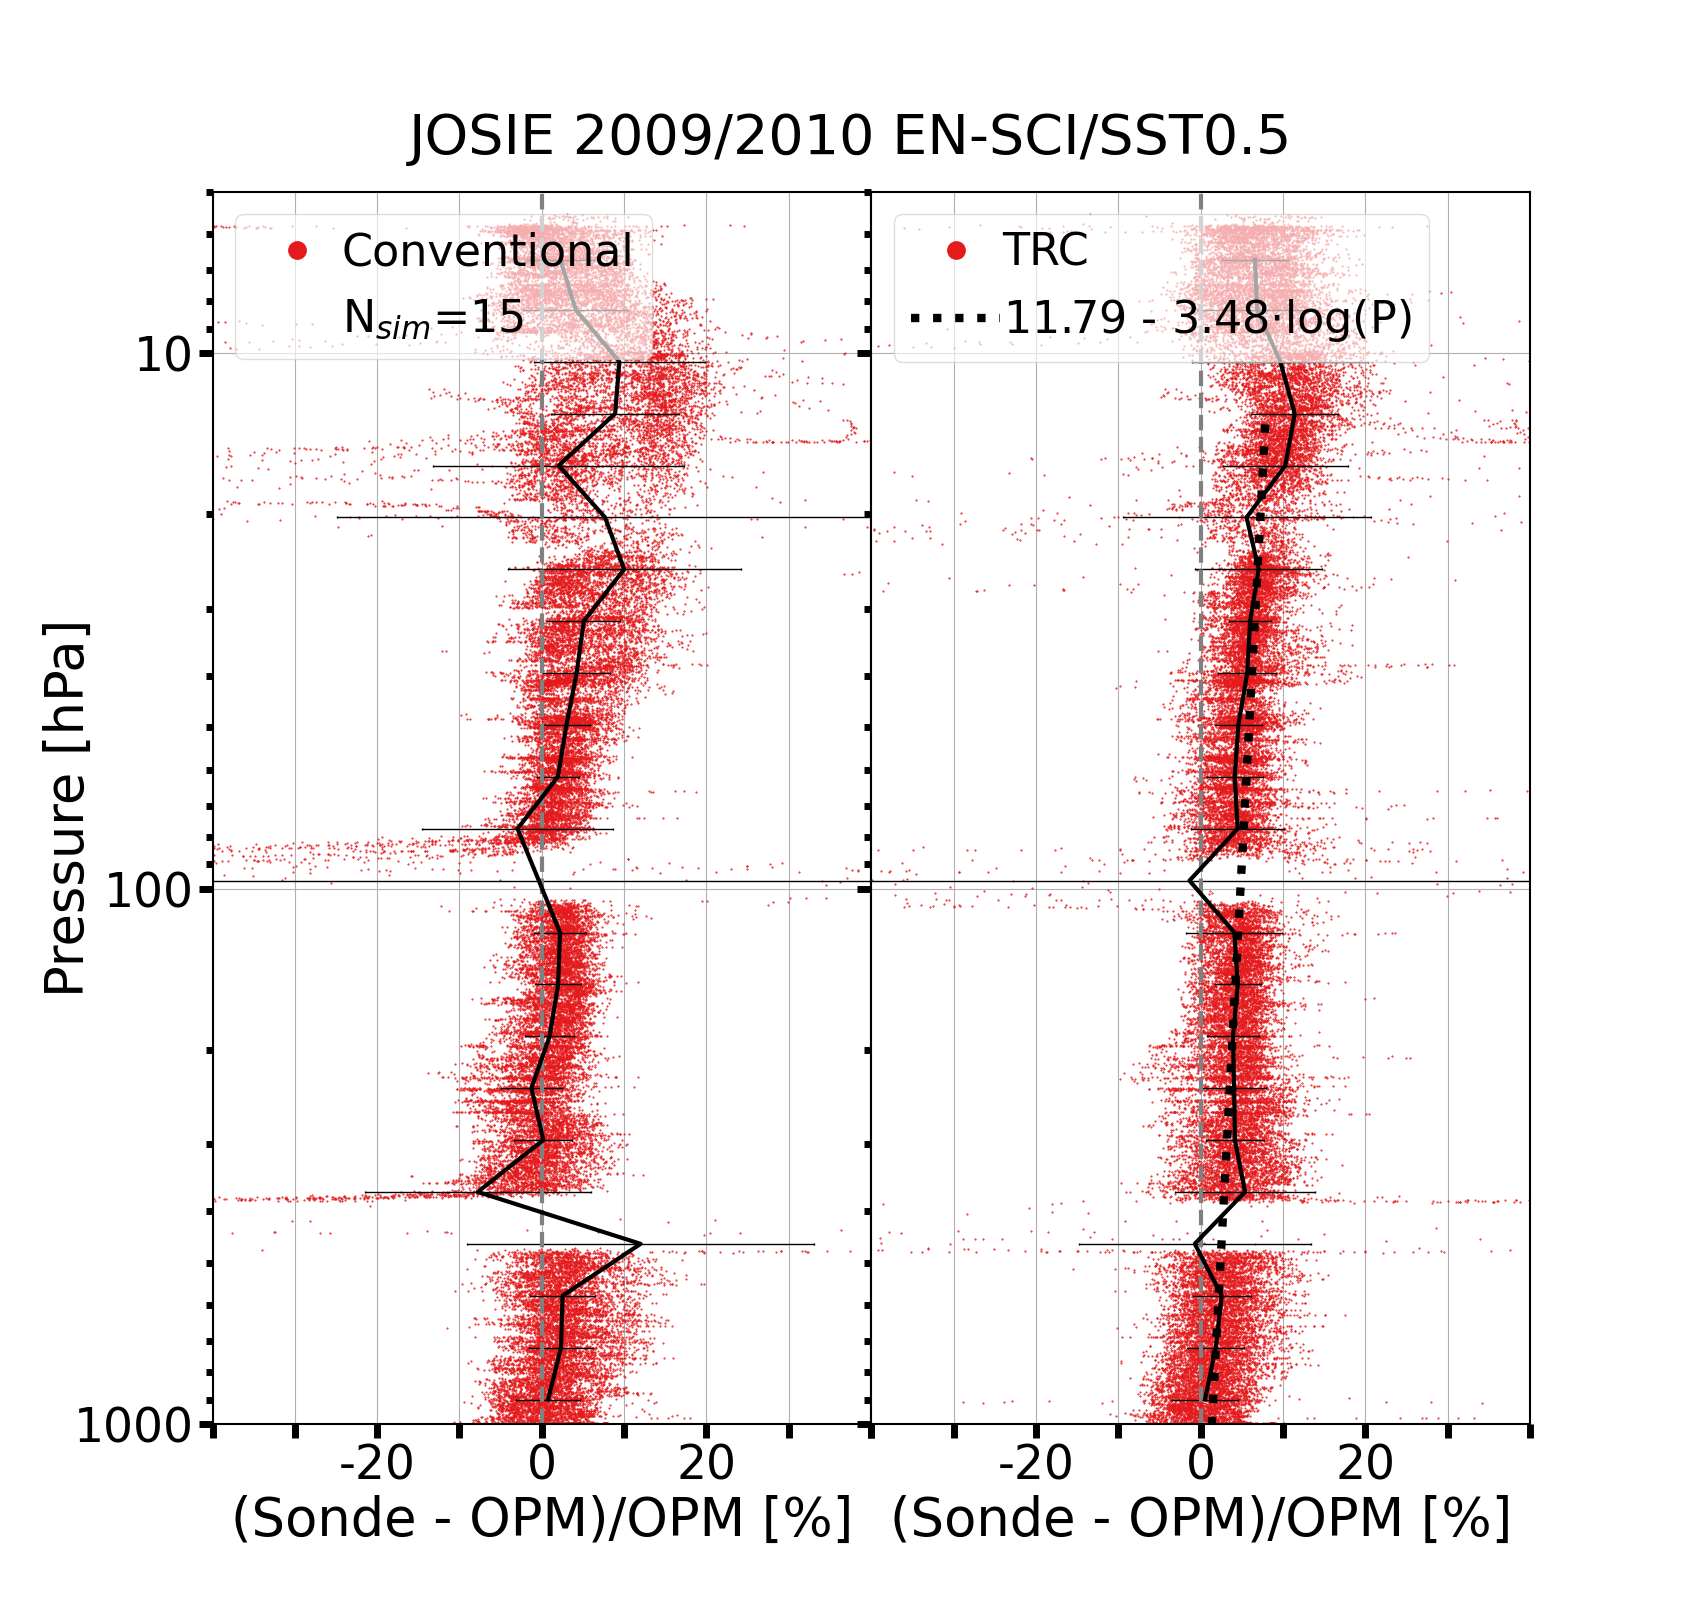
\includegraphics[width=.48\linewidth]{png/scatter_fig6_0910_EN0505_pressure}%
%            \label{subfig:b}%
%        }\\
%        \subfloat[]{%
%            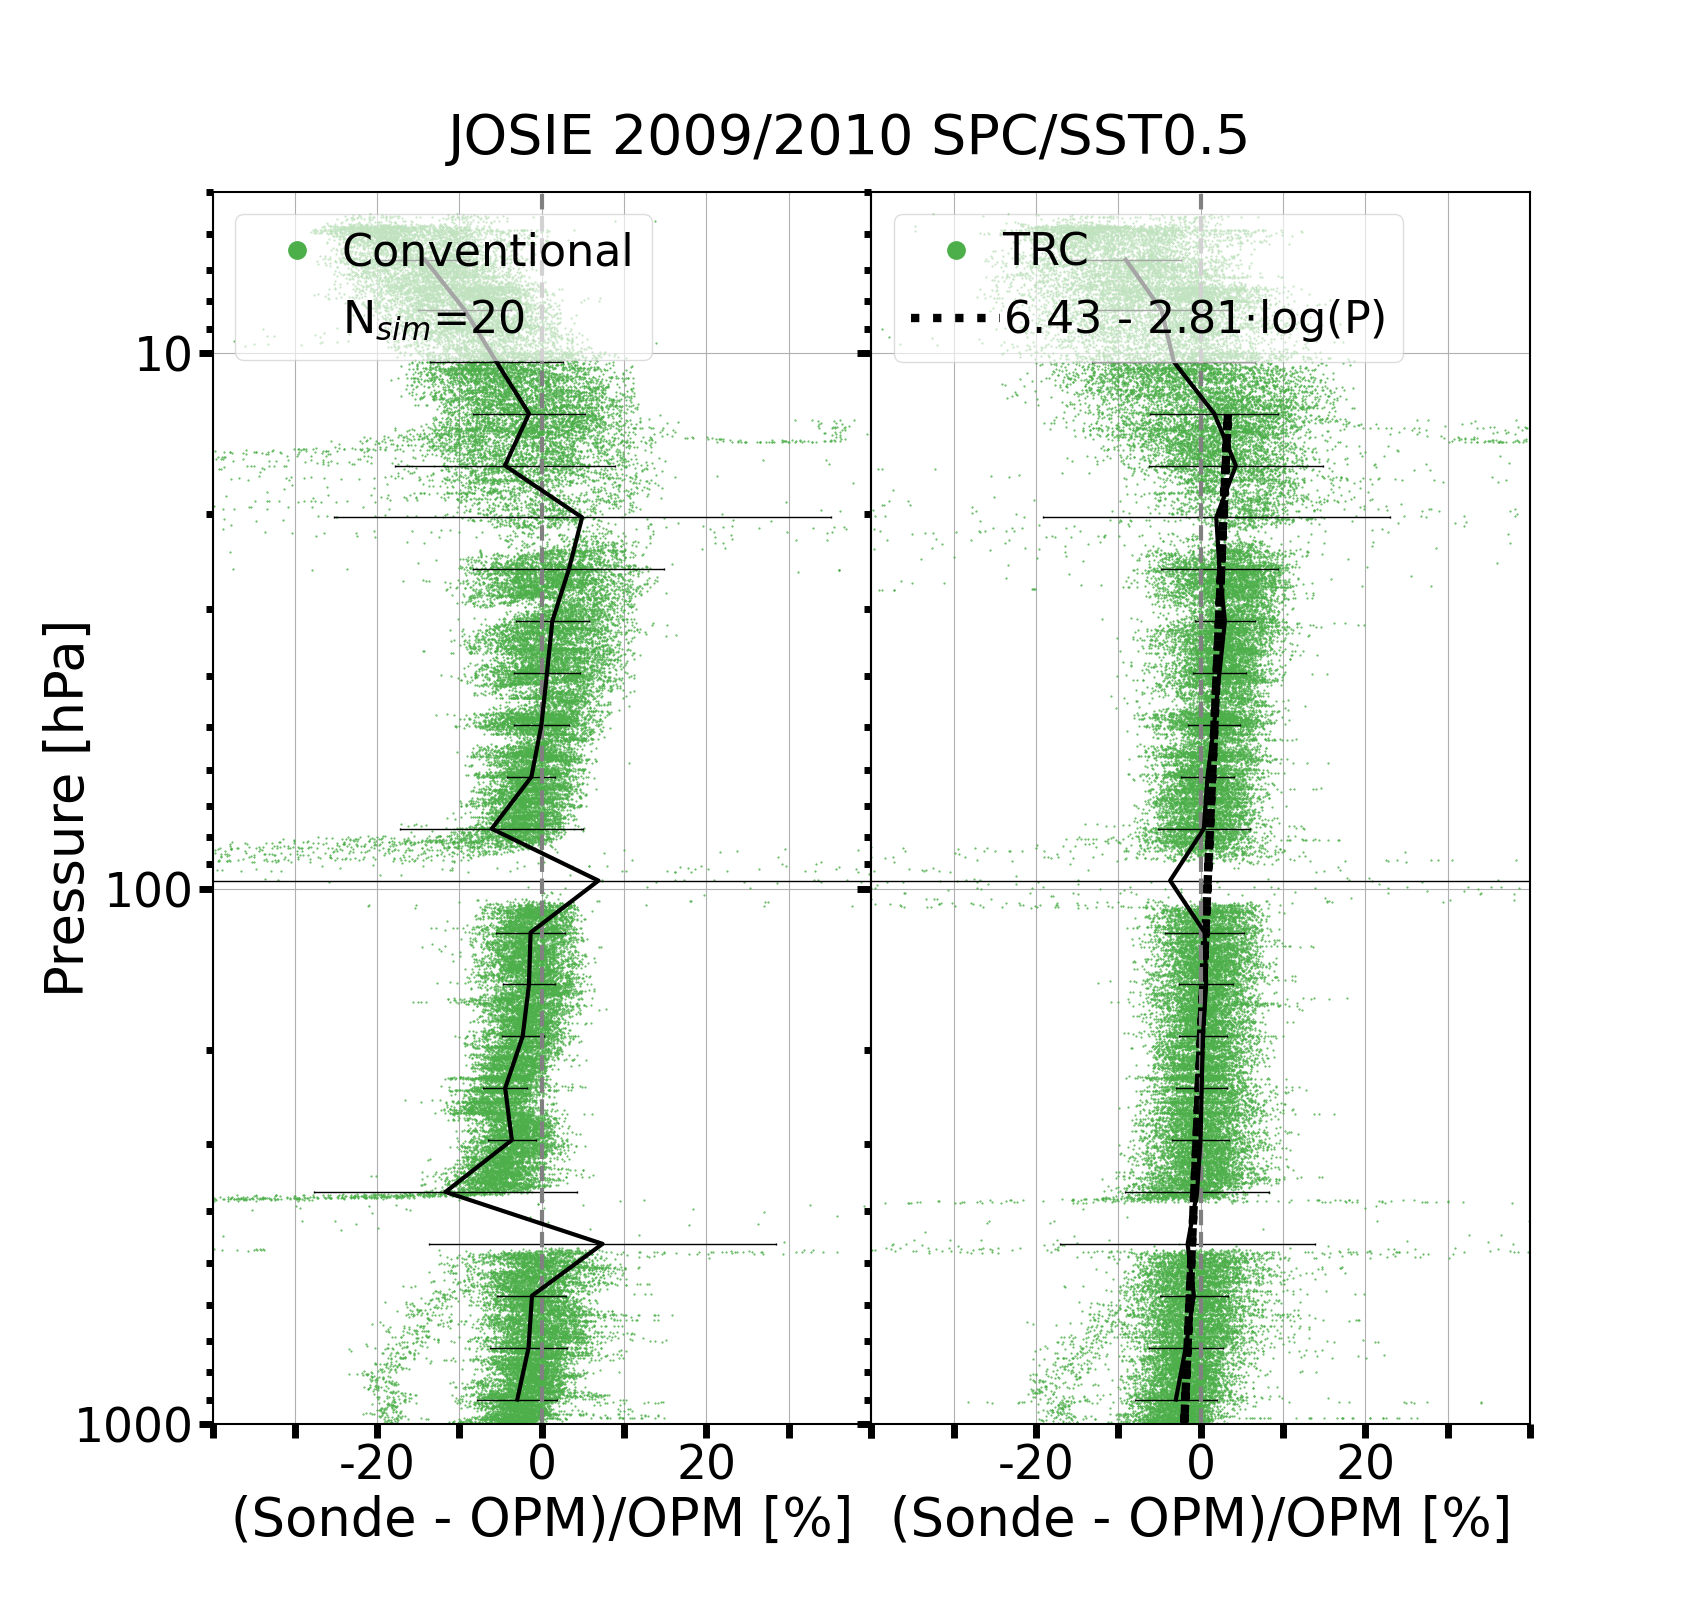
\includegraphics[width=.48\linewidth]{png/scatter_fig6_0910_SPC0505_pressure}%
%            \label{subfig:c}%
%        }\hfill
%        \subfloat[]{%
%            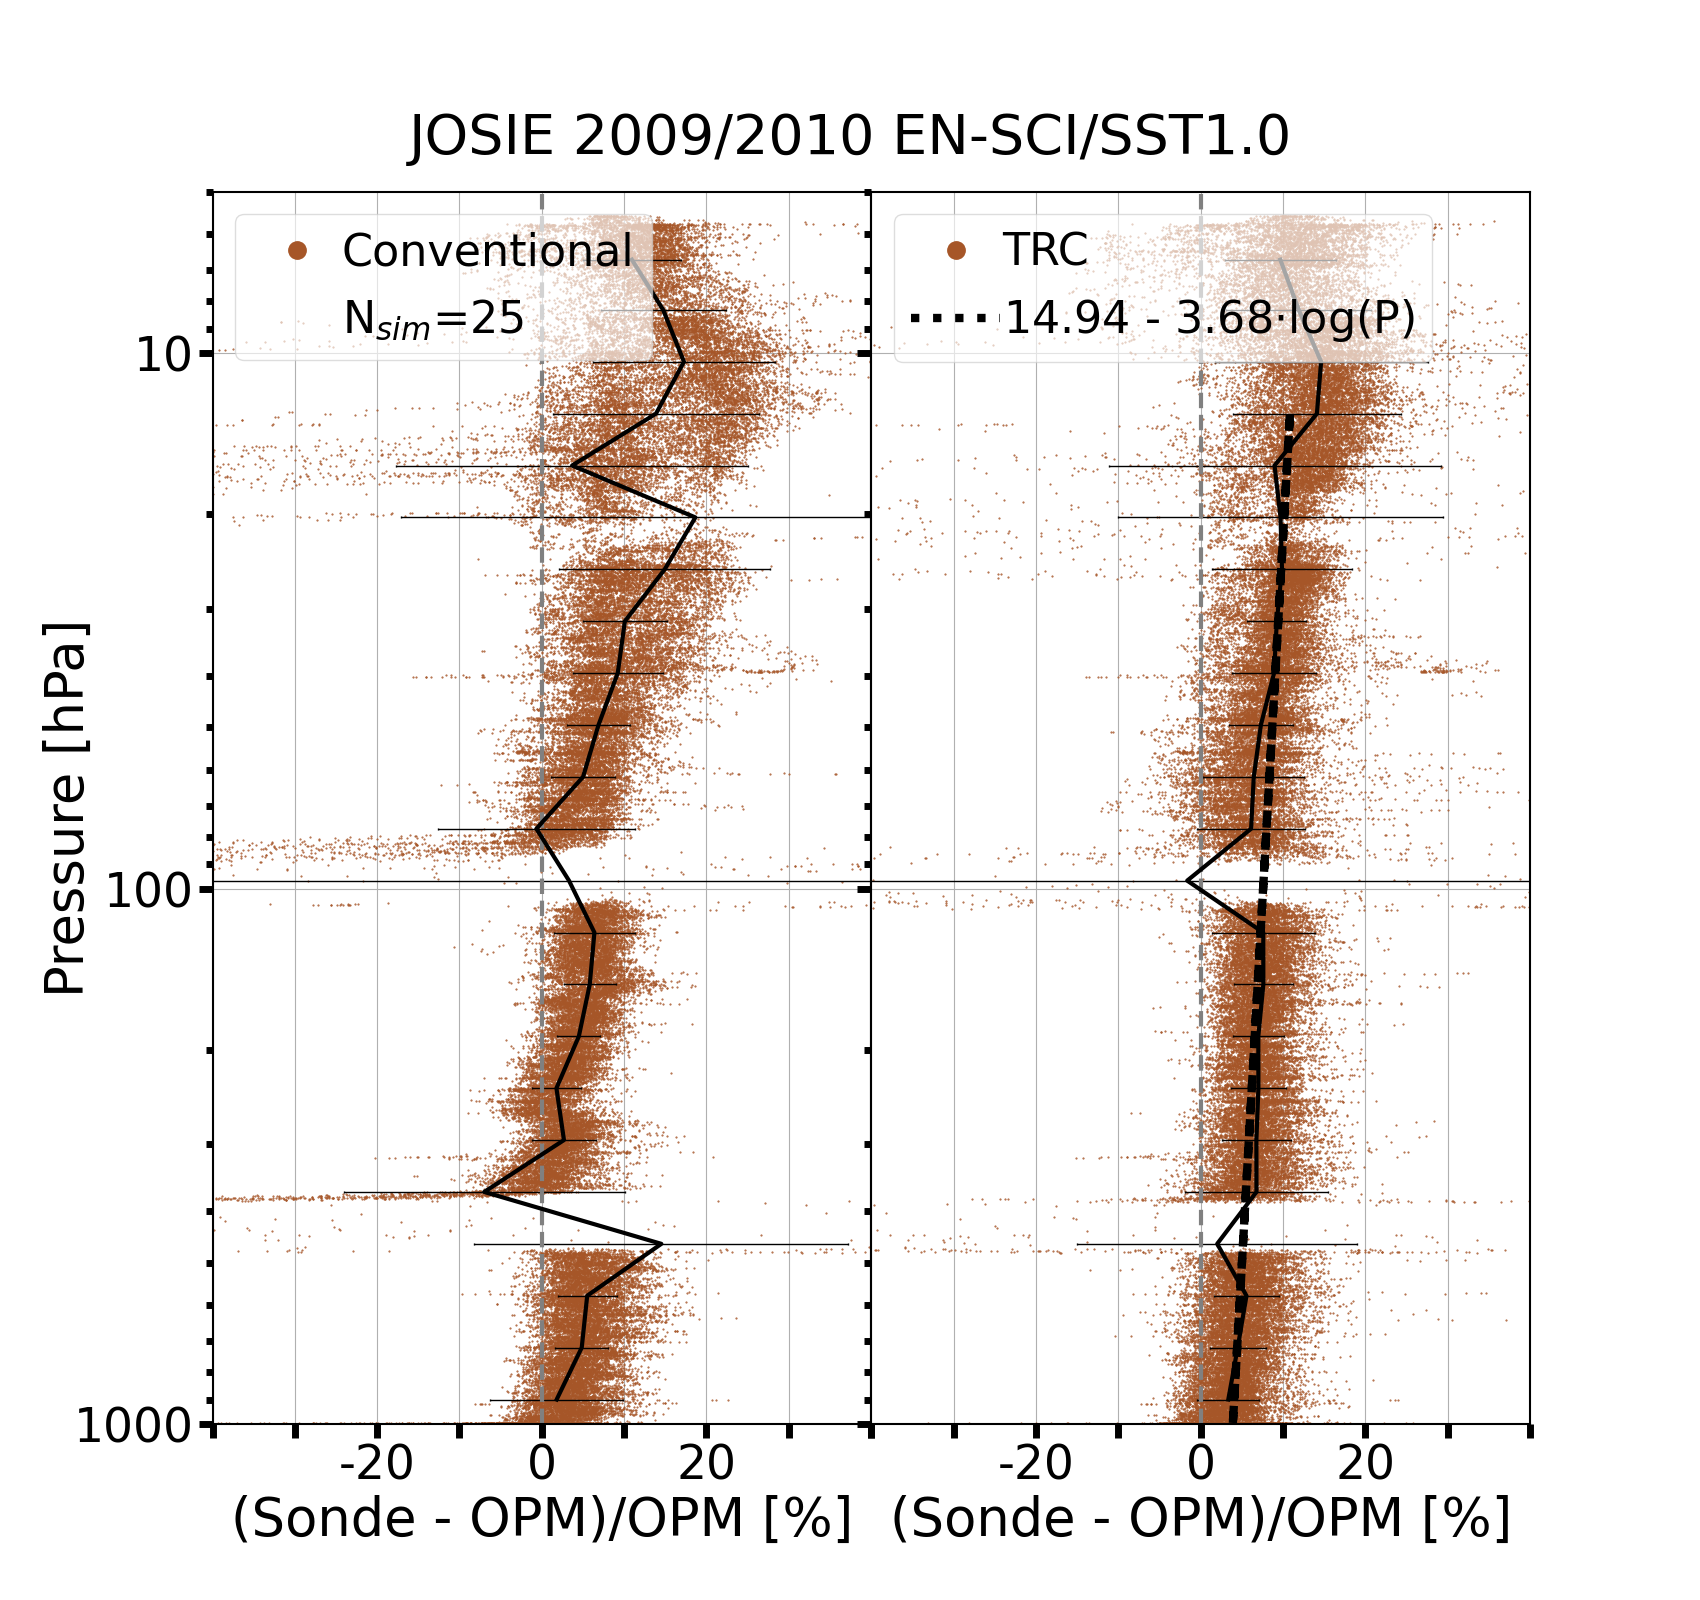
\includegraphics[width=.48\linewidth]{png/scatter_fig6_0910_EN1010_pressure}%
%            \label{subfig:d}%
%        }
%%        \caption{Caption}
%        \label{fig:fig}
%    \end{figure*}
%\end{document}
%
%
%
